\chapter{Results}
\label{chap:results}

\section{Captured images}
16 fps 10 bit synchonized stereo images!


\pagebreak
\begin{figure}[H]
    \centering
    \begin{tabular}[b]{cc}
        \subcaptionbox{Original frame.}{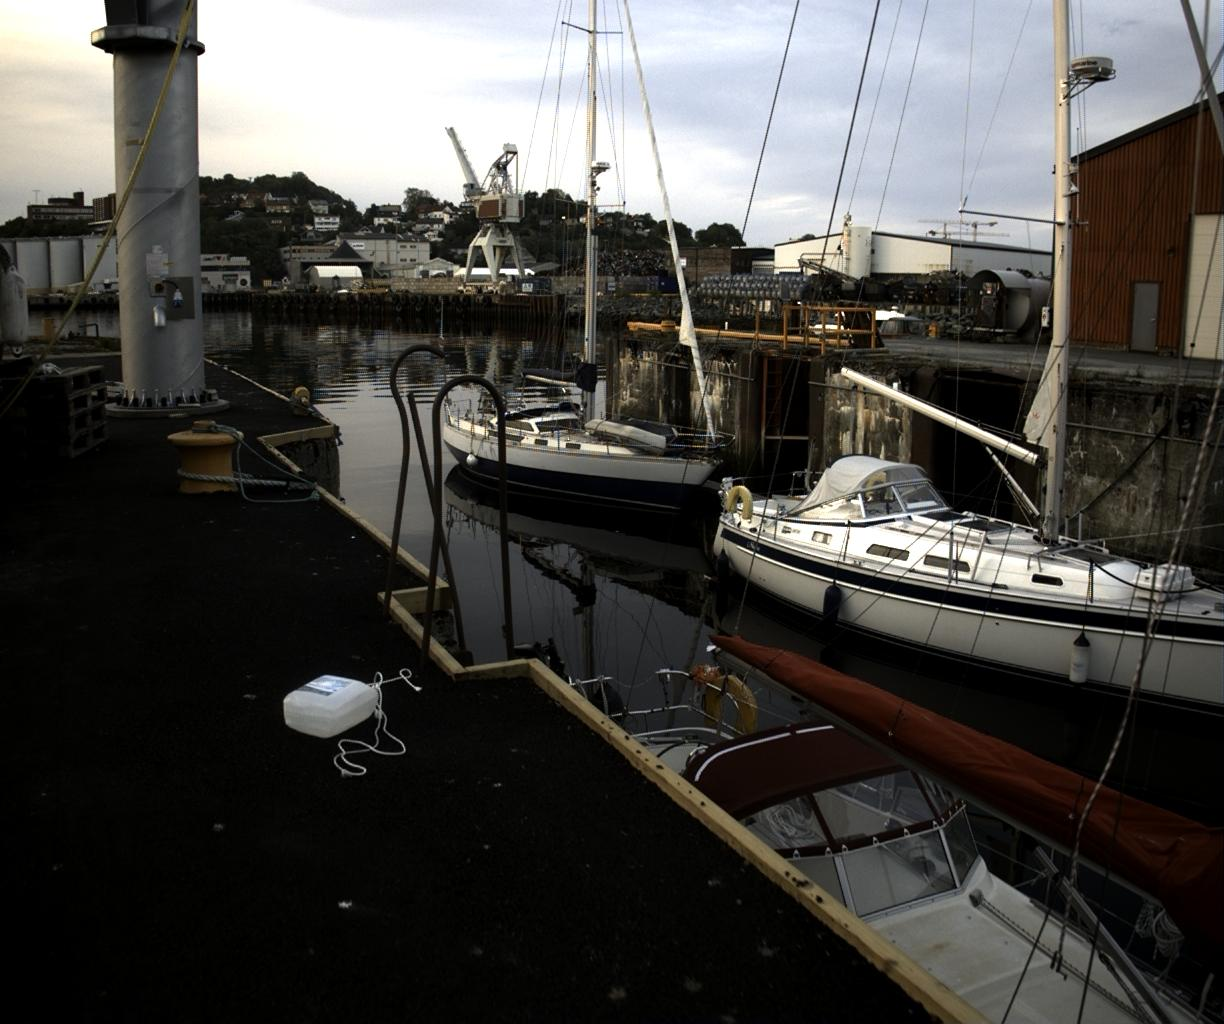
\includegraphics[width=.9\textwidth]{figures/pictures/regular_right_96.jpeg}} \\
        \subcaptionbox{Original frame subtracted from decompressed frame.}{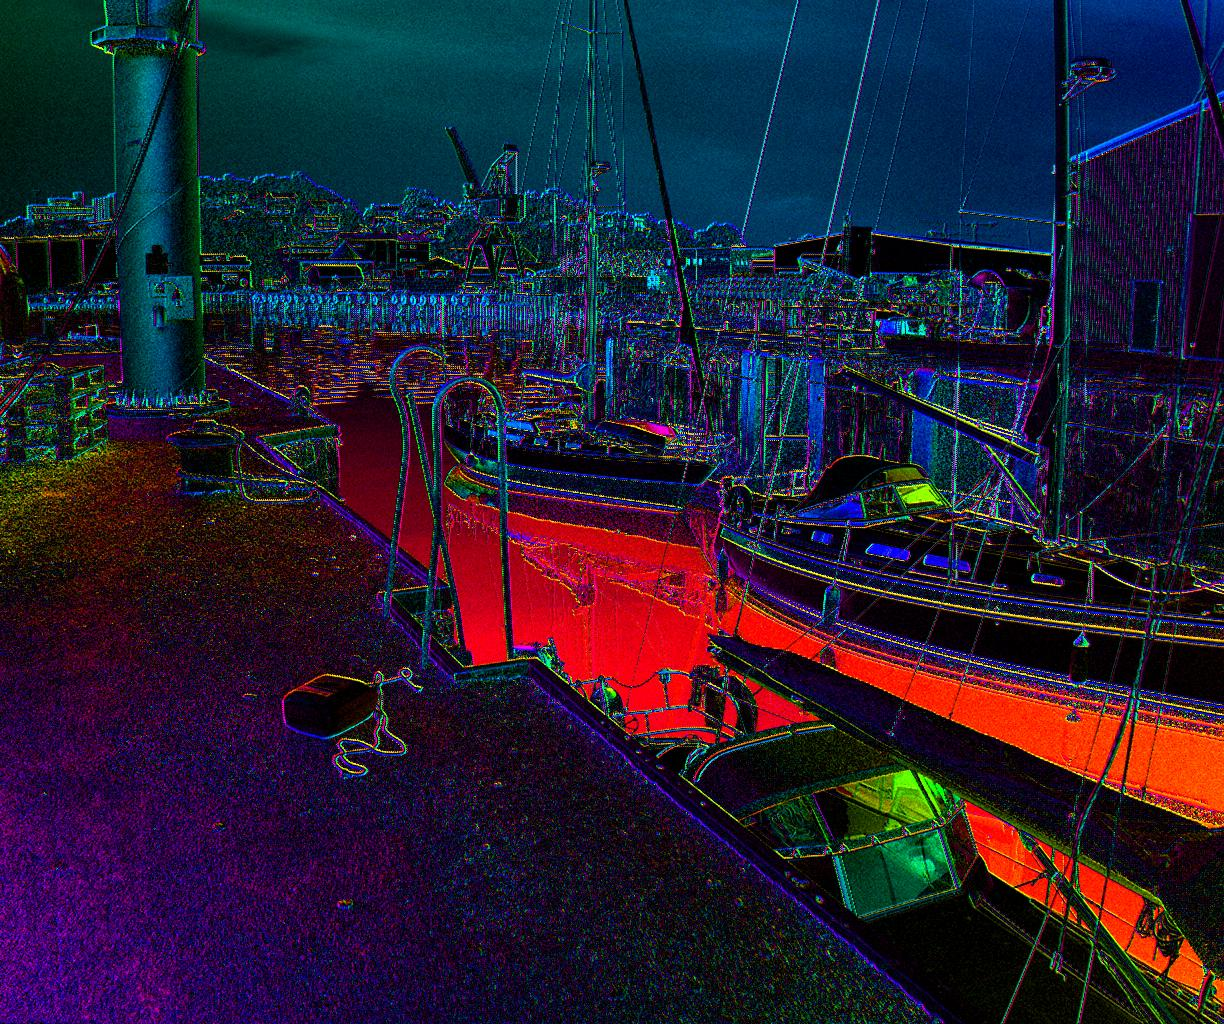
\includegraphics[width=.9\textwidth]{figures/pictures/aolp_right_96.jpeg}}
    \end{tabular}
    \caption{Original frame and compression error revealing use of wrong color profile as brigh regions are too dark and dark regions are too bright.}
\end{figure}

\section{Debayering}
The custom



\section{Compression}



The most efficient video compression method the \jx support is \gls{h265}.

\subsection{Testing method}
To get a rough estiamte of the expected compression performance of the \gls{h265} encoder, a small test was performed.






Without performing any tuning of the compression parameters, the pipeline coppresses the video stream by 75\% on average.


Less than 0.6\% relative error on average at with a 75\% space saving compression ratio.
Possible to acheive better and trade of error for compression ratio.

\subsection{HSV}
Another color representation that is relevant in this \master is \gls{hsv}.
This format is what is usually used when selecting color in a color picker.
A usefull property of this format is that it can be used to easily visualize